\documentclass{beamer}
\mode<presentation>
\usepackage[T1]{fontenc}
\usepackage{tikz}
\usetikzlibrary {calc,graphs,graphs.standard,patterns.meta}
\usepackage{skak}
\usepackage{chessboard}
\usepackage{physics}
\usepackage[dvipsnames]{xcolor}
\definecolor{bgYellow}{HTML}{F0EBDC}
\definecolor{myViolet}{HTML}{403340}

\title{Folds and Graphs}
\author[dishajk]{Disha Kuzhively\\{\scriptsize disha.jk@icts.res.in}\\ICTS-TIFR}
\institute{IdeaLab, VITM Bangalore}
\date[VITM Bangalore]{6 September 2026}
\begin{document}
\setbeamercolor{background canvas}{bg=bgYellow}
\setbeamercolor{title}{fg=myViolet}
\setbeamercolor{frametitle}{fg=myViolet}
\begin{frame}
    \titlepage
\end{frame}
\begin{frame}
    \frametitle{Crane}
\only<2>{       \centering
    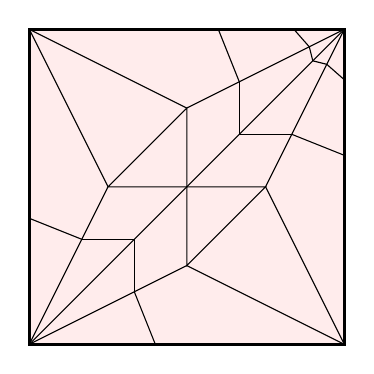
\begin{tikzpicture}
        \coordinate (o) at (0,0);
        \coordinate (l) at (4,4);
        \coordinate (l1) at (4,0);
        \coordinate (l2) at (0,4);
        \coordinate (c) at (2,2);
        \coordinate (a1) at (2,1);
        \coordinate (a2) at (3,2);
        \coordinate (a3) at (2,3);
        \coordinate (a4) at (1,2);
        \coordinate (b1) at ($(o)!2/3!(a1)$);
        \coordinate (b2) at ($(o)!2/3!(a4)$);
        \coordinate (b3) at ($(l)!2/3!(a2)$);
        \coordinate (b4) at ($(l)!2/3!(a3)$);
        \coordinate (b5) at ($(l)!1/3!(b3)$);
        \coordinate (b6) at ($(l)!1/3!(b4)$);
        \coordinate (c1) at ($(o)!2/3!(c)$);
        \coordinate (c2) at ($(l)!2/3!(c)$);
        \coordinate (c3) at ($(l)!1/5!(c)$);
        \coordinate (d1) at ($(o)!4/5!(2,0)$);
        \coordinate (d2) at ($(o)!4/5!(0,2)$);
        \coordinate (d3) at ($(l)!4/5!(4,2)$);
        \coordinate (d4) at ($(l)!4/5!(2,4)$);
        \coordinate (d5) at ($(l)!2/5!(d3)$);
        \coordinate (d6) at ($(l)!2/5!(d4)$);
        \draw[very thick,fill=pink!30] (o) rectangle (l);
        \draw (o) -- (l);
        \draw (o) -- (a1) -- (l1);
        \draw (o) -- (a4) -- (l2);
        \draw (l) -- (a2) -- (l1);
        \draw (l) -- (a3) -- (l2);
        \draw (a1) -- (a2) -- (a4) -- (a3) -- cycle;
        \draw (b1) -- (c1) -- (b2);
        \draw (b3) -- (c2) -- (b4);
        \draw (b1) -- (d1);
        \draw (b2) -- (d2);
        \draw (b3) -- (d3);
        \draw (b4) -- (d4);
        \draw (d5)--(b5) -- (c3) -- (b6) -- (d6);
    \end{tikzpicture}} 
\end{frame}
\begin{frame}
    \frametitle{Recap of Graphs} 
    \begin{columns}[c]
      \begin{column}{0.4\textwidth}
    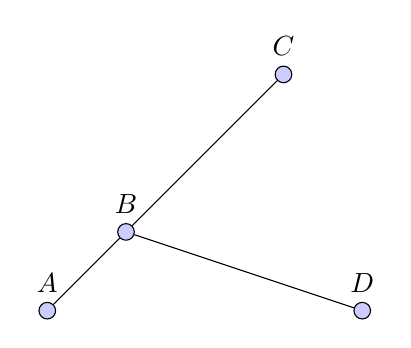
\begin{tikzpicture}
      \graph [
    nodes={
        circle,
        draw,
        fill=blue!20,      % Fills the circle with a color
        minimum size=6pt,  % Reduces the radius/size of the circle
        inner sep=0pt      % Removes internal padding so it stays small
    },
    empty nodes            % Clears the default text from inside the circles
]
{ 
    a[label=above:$A$] -- 
    b[at={(0,1)},label=above:$B$] -- 
    {
        c[at={(1,3)},label=above:$C$], 
        d[at={(2,1)},label=above:$D$]
    } 
};
    \end{tikzpicture}
          \end{column}
      \begin{column}{0.6\textwidth}
    \only<2->{
    \begin{itemize}
    \item $A, B, C, D$ are the \alert{vertices}.
    \item $AB, BC, BD$ are the \alert{edges}.
    \item The number of edges that start at a given vertex is called the \item{degree} of a vertex.
    \end{itemize}
    }
    \only<3->{
      \begin{block}{Question}
      What are the degrees of the vertices $A, B, C, D$?
      \end{block} 
    }
      \end{column}
    \end{columns}
\end{frame}

\end{document}
\begin{frame}
    \centering
    \begin{tikzpicture}
        \only<1>{
        \draw[very thick,fill=pink!30,rotate=45] (0,0) rectangle (4,4);
        \draw[dashed,rotate=45] (0,0) -- (4,4);
        \draw[dashed,rotate=45] (4,0) -- (0,4);}
        \only<2-3>{
        \draw[very thick,rotate=45] (0,0) rectangle (4,4);
            \draw[rotate=45] (0,0) -- (4,4);
        \draw[rotate=45] (4,0) -- (0,4);
                \draw[dashed,rotate=45] (0,2) -- (4,2);
        \draw[dashed,rotate=45] (2,0) -- (2,4);}
        \only<3>{
            \draw[->,rotate=45,xshift=2mm,yshift=-2mm] (4,0) to [out=135,in=45] (0,0); 
        }

    \end{tikzpicture}
\end{frame}